\newpage
\section{Daniel Mazur}
\label{sec:pawljmlo}

Piękne równanie:
\begin{math}
a^2 + b^2 = c^2
\end{math}

\vspace{5mm} %5mm vertical space

Tutaj jest zdjęcie kotka: (Patrz zdjęcie~\ref{fig:kot}).

\begin{figure}[htbp] 
    \centering
    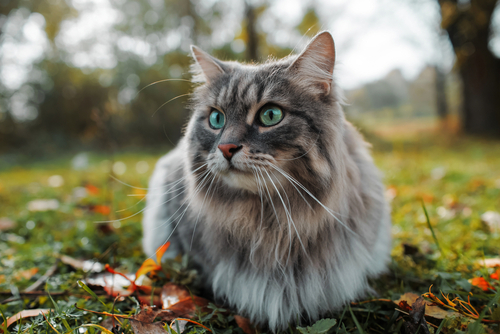
\includegraphics[width=0.4\textwidth]{pictures/kot xd.jpg}
    \caption{To jest kot.}
    \label{fig:kot}
\end{figure}


Tabela~\ref{tab:telefony} reprezentuje popularność danych marek telefonów (nieprawdziwe dane)
\begin{table}[htbp]
\centering
\begin{tabular}{|l|l|l|l|l|}
\hline
\textbf{Ulubione marki telefonów} & Apple & Samsung & Huawei & Xiaomi \\ \hline
Kobiety                           & 10\%  & 45\%    & 20\%   & 25\%   \\ \hline
Męźczyźni                         & 15\%  & 55\%    & 15\%   & 15\%   \\ \hline
Dzieci                            & 30\%  & 40\%    & 10\%   & 20\%   \\ \hline
\end{tabular}
\label{tab:telefony}
\caption{Taka se tabela}
\end{table}

Lista przedmiotów na pierwszym semestrze:
\begin{itemize}
    \item Algebra
    \item Analiza
    \item WDI
    \item KSC
    \item WABIK
    \item WF
    \item Sieci
    \item Prawo karne
\end{itemize}
\newpage
Lista tematów na kolosa z analizy:
\begin{enumerate}
    \item Zbiory
    \item Funkcje
    \item Ciągi
\end{enumerate}

\begin{center}
\section*{Inwokacja}

\emph{Litwo!} Ojczyzno \underline{moja}! ty jesteś jak zdrowie.\\
Ile \textbf{cię} trzeba cenić, ten tylko się dowie,\\

Kto cię \emph{stracił}. Dziś piękność twą w całej ozdobie\\
Widzę i opisuję, bo \underline{tęsknię} po tobie.\\
\end{center}


